\begin{figure}[H]
\centering
\begin{tabular}{CCC}
    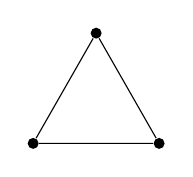
\begin{tikzpicture}[every node/.style={circle,fill,inner sep=1.4pt}]
    \node (a) at (0,0.9) {};
    \node (b) at (-0.8,-0.5) {};
    \node (c) at (0.8,-0.5) {};
    \draw (a)--(b)--(c)--(a);
    \end{tikzpicture}
&
    \begin{ZX}[circuit,mbr=3]
        \zxInput{\ket0} \ar[r] & \zxCross{} \ar[d] \rar & \zxCross{} \ar[dd] \rar & \rar & \\
        \zxInput{\ket0} \ar[r] & \zxCross{} \rar & \rar & \zxCross{} \ar[d] \rar & \\
        \zxInput{\ket0} \ar[r] & \rar & \zxCross{} \rar & \zxCross{} \rar &
    \end{ZX}
&
    \begin{ZX}[mbr=3]
        \zxZ{} \ar[r,hw] & \zxZ{} \ar[d,hw] \rar & \zxZ{} \ar[dd,hw] \rar & \rar & \\
        \zxZ{} \ar[r,hw] & \zxZ{} \rar & \rar & \zxZ{} \ar[d,hw] \rar & \\
        \zxZ{} \ar[r,hw] & \rar & \zxZ{} \rar & \zxZ{} \rar &
    \end{ZX}
\end{tabular}
\caption{The triangle graph and its circuit and ZX graph state.}
\label{fig:triangle-graph}
\end{figure}